\documentclass{math}

\usepackage{graphicx}

\title{Introduction to Cryptography}
\author{Alvin Lin}
\date{January 2018 - May 2018}

\begin{document}

\maketitle

\section*{Polynomial Arithmetic}

\subsection*{Finite Fields of the Form \( GF(p^m) \)}
\textbf{Galois' Theorem:} An order-\textit{n} finite field exists if and only if
\( n = p^m \) for some prime \( p \) and some positive integer \( m \).
\begin{itemize}
  \item \( p \) is called the characteristic of this finite field.
  \item The order of a finite field is its number of elements.
  \item We use \( GF(p^m) \) or \( \mathbb{F}_{p^m} \) to represent the finite
  field of order \( p^m \).
  \item An order-\textit{n} finite field is unique (up to isomorphism).
  \item Addition and multiplication module a prime number \( p \) form a finite
  field \( \Z_p = GF(p) \).
  \item If \( m = 1 \), then \( \Z_p = GF(p) \)
  \item One way to construct a finite field with \( m > 1 \) is using the
  polynomial basis. The field is constructed as a set of \( p^m \) polynomials
  along with two polynomial operations.
\end{itemize}

\subsection*{Polynomial Arithmetic}
A polynomial \( f(x) \) is a mathematical expression of the form:
\[ a_nx^n+a_{n-1}x^{n-1}+\dots+a_0 \]
The highest exponent of \( x \) is the degree of the polynomial. \( a_n,
a_{n-1}, \dots, a_0 \) are called coefficients. We can add, subtract, multiply,
and divide polynomials. AES is a byte oriented cipher where 1 byte can be
represented as a 7th degree polynomial.
\par All arithmetic can be done in the Galois field \( GF(2^8) \). If a
polynomial is divisible only by itself and constants, then we call this
polynomial an irreducible polynomial. \( gcd(a(x), b(x)) \) is the polynomial
of maximum degree that divides both \( a(x) \) and \( b(x) \). Similar to
integers, you can do modular arithmetic with polynomials over a field. Now the
operands and modulus are polynomials.

\subsection*{Revisiting Block Ciphers}
A block cipher is much more than just an encryption algorithm, it can be used
\begin{itemize}
  \item to build different types of block-based encryption schemes
  \item to realize stream ciphers
  \item to construct hash functions
  \item to make message authentication codes
  \item to build key establishment protocols
  \item to make a pseudo-random number generator
\end{itemize}
Block cipher security can be increased by key whitening or multiple encryption.
There are several ways of encrypting long plaintexts with a block cipher:
\begin{itemize}
  \item Electronic Code Book mode (ECB)
  \item Cipher Block Chaining mode (CBC)
  \item Output Feedback mode (OFB)
  \item Cipher Feedback mode (CFB)
  \item Counter mode (CTR)
  \item Galois Counter Mode (GCM)
\end{itemize}
These modes have the goal of providing authenticity and integrity in addition to
confidentiality. It ascertains that the message is coming from the original
sender and that it was not altered during transmission.

\subsubsection*{Electronic Code Book mode (ECB)}
This is the simplest of the encryption modes. Messages which exceed \textit{b}
bits are partitioned into \textit{b}-bit blocks, which are encrypted separately.
In case the plaintext message's length is not a multiple of \textit{b}, we add
padding to the end.
\begin{center}
  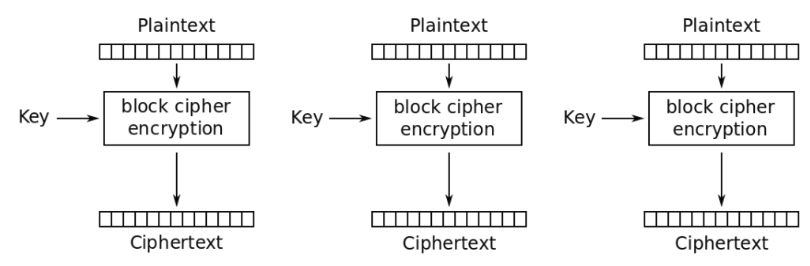
\includegraphics[width=12cm]{assets/ecb.png}
\end{center}
\textbf{Advantages:}
\begin{itemize}
  \item No block synchronization between the sender and receiver is required.
  \item Bit errors caused by noisy channels only affect the corresponding block
  but not succeeding blocks.
  \item Encryption can be parallelized, which is an advantage for high-speed
  implementations.
\end{itemize}
\textbf{Disadvantages:}
\begin{itemize}
  \item Encryption is highly deterministic.
  \item Identical plaintexts result in identical ciphertexts.
  \item An attacker recognizes if the same message has been sent twice.
  \item Plaintext blocks are encrypted independently of previous blocks.
  \item An attacker may reorder ciphertext blocks which result in valid
  plaintext.
  \item Statistical properties in the plaintext are preserved in the
  ciphertext.
\end{itemize}
Once a particular plaintext to ciphertext block mapping is known, a sequence of
ciphertext blocks can easily be manipulated.

\subsubsection*{Cipher Block Chaining mode (CBC)}
There are two main ideas behind this mode: the encryption of all blocks are
chained together, and the encryption is randomized by using an initialization
vector.
\begin{center}
  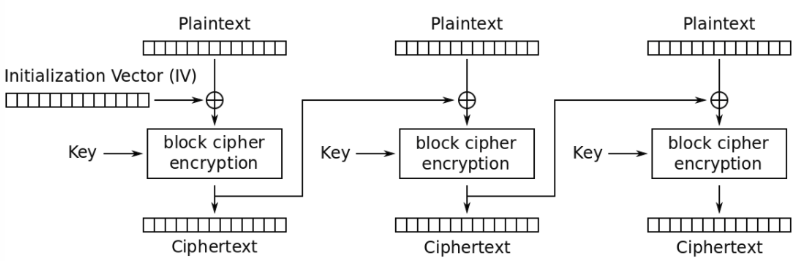
\includegraphics[width=12cm]{assets/cbc.png}
\end{center}
This mode also requires padding, but messages longer than \( 2^{\frac{n}{2}} \)
blocks (where \( n \) is the block size in bits) shouldn't be encrypted with
this mode, since it gives an attacker more information about the ciphertext.
Encryption cannot be parallelized, but decryption can be. The initialization
vector does not need to be secret, but it should be a randomized nonce.

\subsubsection*{Output Feedback mode (OFB)}
This mode builds a synchronous stream cipher from a block cipher, where the key
stream is generated in a blockwise fashion. The output of the cipher gives us
key stream bits with which we can encrypt plaintext bits using the XOR
operation. This mode also requires an initialization vector (which also should
be a randomized nonce).
\begin{center}
  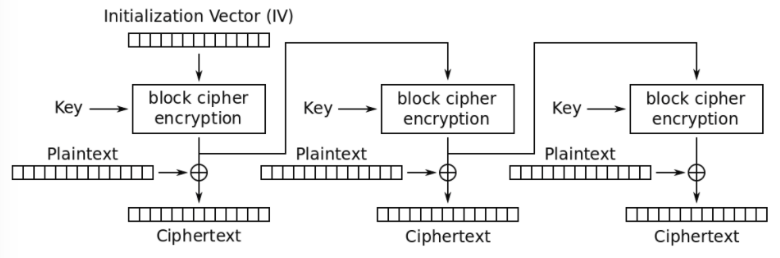
\includegraphics[width=12cm]{assets/ofb.png}
\end{center}

\subsubsection*{Cipher Feedback mode (CFB)}
This mode uses a block cipher as a building block for an synchronous stream
cipher. The key stream is generated in a blockwise fashion and is also a
function of the ciphertext. Since it also uses a randomized initialization
vector, the ciphertext is also nondeterministic. It can be used in situations
where short plaintext blocks are to be encrypted, but has no real advantage
over Output Feedback mode.
\begin{center}
  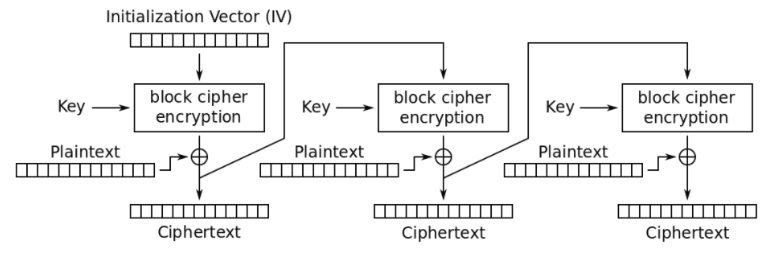
\includegraphics[width=12cm]{assets/cfb.png}
\end{center}

\subsubsection*{Counter mode (CTR)}
This mode turns a block cipher into a stream cipher where the keystream is
computed in a blockwise fashion (similar to OFB and CFB mode). The input to the
block cipher is a counter which assumes a different value every time the block
cipher computes a new key stream block. Unlike CFB, and OFB however, this is
highly parallelizable and does not require padding since the unneeded portion
of the last key block can be discarded (because it is a stream cipher).
\begin{center}
  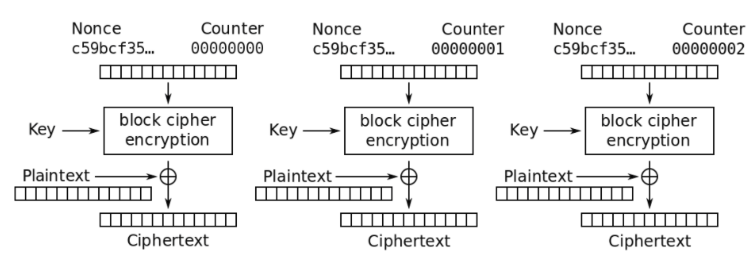
\includegraphics[width=12cm]{assets/ctr.png}
\end{center}

\section*{Exhaustive Key Search}
A simple exhaustive search for a DES key pair knowing one plaintext-ciphertext
pair requires has a key space of size \( 2^56 \). However, for most other block
ciphers, a key search is somewhat more complicated. A brute-force attack can
produce false positive results, where a key is found that is not the one used
for the encryption. The likelihood of this is related to the relative size of
the key space and the plaintext space.

\subsubsection*{Example}
Assume a cipher with a block width of 64 bits and a key size of 80 bits is used
to encrypt a plaintext. If we encrypt once under all possible \( 2^80 \) keys,
we obtain \( 2^80 \) possible ciphertexts. However, there exist only \( 2^64 \)
different ones. If we run through all keys for a given plaintext-ciphertext
pairs, we find on average \( \frac{2^80}{2^64} = 2^16 \) keys that perform the
mapping \( e_k(x) = y \). Given a block cipher with a key length of \( k \)
bits and a block size of \( n \) bits, as well as \( t \) plaintext-ciphertext
pairs, the expected number of false keys which encrypts all plaintexts to the
corresponding ciphertexts is:
\[ 2^{k-tn} \]

\begin{center}
  You can find all my notes at \url{http://omgimanerd.tech/notes}. If you have
  any questions, comments, or concerns, please contact me at
  alvin@omgimanerd.tech
\end{center}

\end{document}
